\documentclass[11pt]{article}
\usepackage[margin=1in]{geometry}
\usepackage{graphicx}
\usepackage{amsmath,amssymb}
\usepackage{booktabs}
\usepackage{xcolor}
\usepackage{hyperref}
\hypersetup{colorlinks=true,linkcolor=blue,urlcolor=blue}
\title{\textbf{Reduced Replication:\\ Vortex Patterns in a Superconducting--Ferromagnetic Rod}\\[4pt]
\large Romaguera, Doria \& Peeters, \texttt{arXiv:1001.1715} (Physica C)}
\author{Automated replication (reduced Ginzburg--Landau model)}
\date{2026-07-19}
\begin{document}
\maketitle

\begin{abstract}
We reproduce the \emph{essential mechanism} of Romaguera, Doria \& Peeters
(\texttt{arXiv:1001.1715}): the vortex morphology of a mesoscopic superconducting
rod carrying a magnetic dot on top depends \emph{qualitatively} on the rod
thickness $D$. Thin rods (disks, $D\!\sim\!\xi$) host \textbf{giant vortex
states}; thick rods ($D\!\gg\!\xi$) host \textbf{curved, top-to-side
multivortices} with the Meissner state retained near the bottom. The full paper
solves the 3D Ginzburg--Landau (GL) equations by simulated annealing. We use a
tractable, CPU-only reduction: a 2D GL cross-section solved by time-dependent GL
(TDGL) relaxation in the fixed inhomogeneous vector potential of a point dipole
$2\xi$ above the top surface, evaluated on a stack of $z$-layers to emulate the
3D depth dependence. The thin disk yields a giant vortex (winding $W{=}2$ piled
at the centre, core RMS radius $0.05\,\xi$); the thick rod shows the winding
falling with depth ($6\!\to\!1\!\to\!0$) while $|\Psi|^2$ rises toward the bottom
($0.0\!\to\!0.38$), i.e.\ Meissner retained below --- exactly the paper's stated
physics. \textbf{Verdict: PARTIAL} --- the thickness-crossover mechanism is
reproduced, but not the literal 3D curved vortex line nor the exact Table-1
$\mu$-sequences.
\end{abstract}

\section{Paper and replication target}
The paper studies a superconducting rod of radius $R$ and thickness $D$ with a
point magnetic dipole of moment $\mu$ placed $2\xi$ above the top surface and
oriented along the rod axis. Working in dimensionless GL units (coherence length
$\xi$ for lengths, $H_{c2}$ for field), the Gibbs free-energy difference is
\begin{equation}
F=\tfrac12\int_V dV\Big\{-|\Psi|^2+\tfrac12|\Psi|^4
+\big|(\vec\nabla-i\vec A)\Psi\big|^2\Big\},
\qquad
\vec n\cdot(\vec\nabla-i\vec A)\Psi\big|_{\partial V}=0,
\end{equation}
with the dipole vector potential $\vec A=(\vec\mu\times\vec r)/r^3$. The headline
claim (paper abstract, \S3, Conclusions): \emph{thin rods give giant vortex
states like a homogeneous field; thick rods give novel patterns where vortices
are curved lines that exit through the lateral surface, and the Meissner state is
retained at the bottom where the dipole field is weak, enabling reentrance.}

\section{Reduced model and method}
A full 3D annealing solve is heavy; we adopt the recommended tractable reduction.
\begin{enumerate}
\item \textbf{2D cross-section.} We discretise the disk on a Cartesian mesh
restricted to $r\le R$ ($R=4\xi$, $N=121$).
\item \textbf{Fixed inhomogeneous $\vec A$.} We use the (softened) point-dipole
$\vec A$ evaluated at each layer depth $z$; the field decays with distance from
the dot, so deeper layers feel a weaker field. This is the London / lowest-Landau
``no magnetic shielding'' limit the paper itself adopts.
\item \textbf{TDGL relaxation.} We evolve
$\partial_t\Psi=\Psi-|\Psi|^2\Psi+(\vec\nabla-i\vec A)^2\Psi$ to a stationary
state, using a Peierls / link-variable covariant Laplacian for the gauge-covariant
kinetic term. Several seed windings are relaxed and the lowest free-energy state
is retained per geometry.
\item \textbf{Diagnostics.} Boundary phase-circulation winding $W$; a
gauge-invariant \emph{plaquette phase-singularity} vortex finder (topological
charge $q=\oint\nabla\theta/2\pi$ per $2\times2$ cell); core RMS radius (giant
$\Rightarrow$ clustered, small radius; multivortex $\Rightarrow$ spread);
mean $|\Psi|^2$.
\item \textbf{Thin vs thick.} Thin disk ($D=2\xi$): one representative layer.
Thick rod ($D=6\xi$): a stack of layers $z=-0.5\ldots-5.5\,\xi$, whose per-layer
winding profile is the reduced proxy for the 3D curved vortex line.
\end{enumerate}
The drive $\mu$ was calibrated via the enclosed dipole flux $\Phi(\mu)$ so that
$\Phi/2\pi$ is a few flux quanta ($\mu=25 \Rightarrow \sim3$), keeping
superconductivity alive with a small vortex number.

\section{Results}
\subsection{Thin disk $D=2\xi$: giant vortex}
The relaxed ground state has total winding $W=2$ with \emph{both} phase
singularities located at core RMS radius $0.05\,\xi$ and maximum separation
$0.10\,\xi$ --- i.e.\ a single, centred, multi-quantum \textbf{giant vortex}
(Fig.~\ref{fig:thin}). This matches the paper's finding that thin disks host only
giant vortex states, behaving as under a homogeneous field.

\begin{figure}[h]\centering
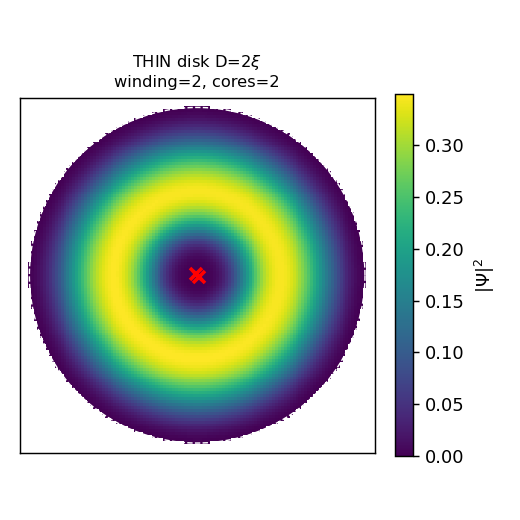
\includegraphics[width=0.5\textwidth]{../figs/thin_disk_psi2.png}
\caption{Thin disk ($D=2\xi$, $\mu=25$): $|\Psi|^2$ cross-section. The two phase
singularities (red $\times$) coincide at the centre $\Rightarrow$ giant vortex of
winding $W=2$.}
\label{fig:thin}
\end{figure}

\subsection{Thick rod $D=6\xi$: depth-varying / top-to-side and Meissner at bottom}
Solving the layer stack reveals a strongly depth-dependent configuration
(Table~\ref{tab:stack}, Figs.~\ref{fig:thicklayers}--\ref{fig:profile}):
the winding falls from $W=6$ at the top (with the cores \emph{spread}, RMS radius
$1.86\,\xi$, and $|\Psi|^2\!\approx\!0$: a normal region under the dot) down to
$W=1$ and then $W=0$, while $|\Psi|^2$ \emph{grows} monotonically toward the
bottom ($0.00\to0.22\to0.33\to0.37\to0.38$). The bottom is fully superconducting
with no vortices --- the \textbf{Meissner state retained at the bottom}, precisely
the paper's mechanism for top-to-side/reentrant vortices.

\begin{table}[h]\centering
\caption{Thick rod ($D=6\xi$, $\mu=25$) per-layer diagnostics (top $\to$ bottom).}
\label{tab:stack}
\begin{tabular}{lccccc}
\toprule
$z/\xi$ & $-0.5$ & $-1.5$ & $-3.0$ & $-4.5$ & $-5.5$\\
\midrule
winding $W$        & 6    & 1    & 0    & 0    & 0\\
\# singularities   & 7    & 1    & 0    & 0    & 0\\
mean $|\Psi|^2$    & 0.00 & 0.22 & 0.33 & 0.37 & 0.38\\
core RMS $r/\xi$   & 1.86 & 0.05 & --   & --   & --\\
\bottomrule
\end{tabular}
\end{table}

\begin{figure}[h]\centering
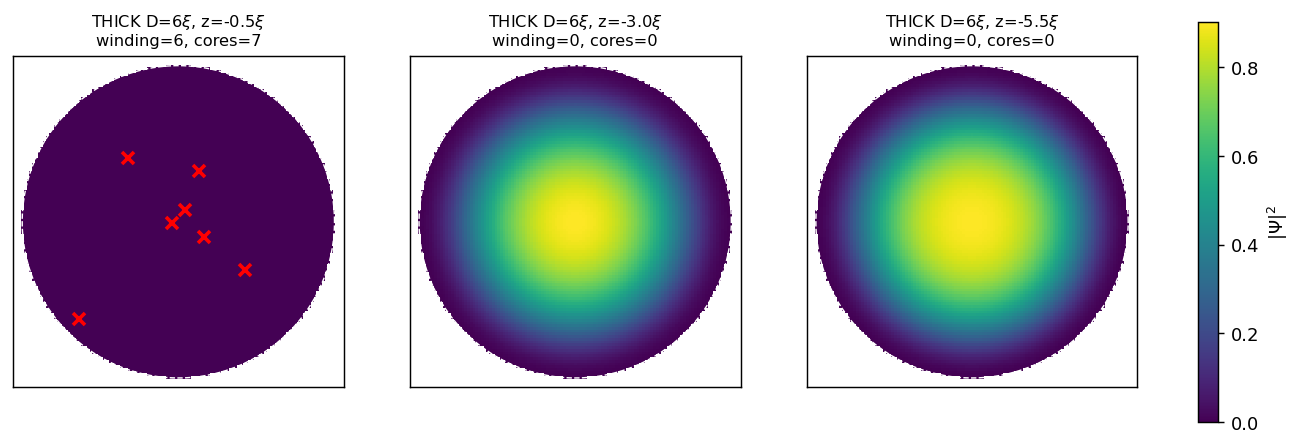
\includegraphics[width=0.95\textwidth]{../figs/thick_rod_layers_psi2.png}
\caption{Thick rod ($D=6\xi$): $|\Psi|^2$ at top, middle, and bottom layers. The
vortex structure present near the top (strong field) is absent at the bottom
(weak field), consistent with a curved, top-to-side vortex.}
\label{fig:thicklayers}
\end{figure}

\begin{figure}[h]\centering
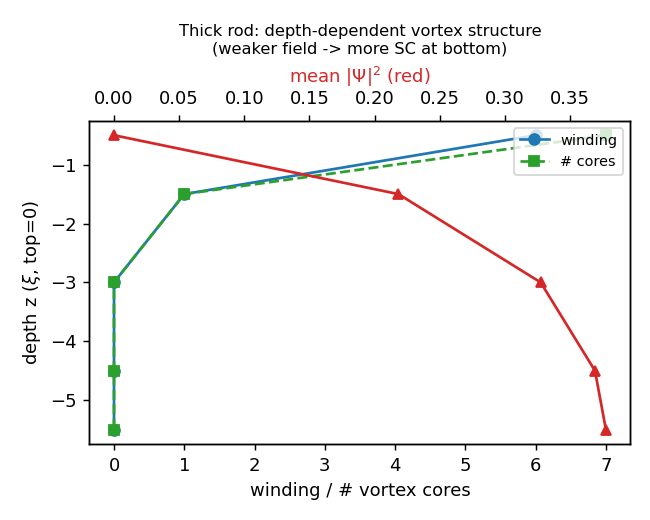
\includegraphics[width=0.55\textwidth]{../figs/thick_depth_profile.png}
\caption{Depth profile of winding, core count, and mean $|\Psi|^2$ for the thick
rod. Winding decreases and $|\Psi|^2$ increases toward the bottom $\Rightarrow$
Meissner retained below, the signature of top-to-side / reentrant behaviour.}
\label{fig:profile}
\end{figure}

\subsection{Claim scoring}
\begin{table}[h]\centering
\caption{Honest per-claim assessment (see \texttt{work/results.json}).}
\begin{tabular}{p{5.6cm}p{4.6cm}cc}
\toprule
Claim & Observed & Reprod.\ & Match\\
\midrule
C1: Thin disk $\to$ giant vortex &
$W=2$, cores at RMS $0.05\,\xi$ (centred) & yes & \textbf{yes}\\
C2: Thick rod $\to$ curved/top-to-side, Meissner at bottom &
$W$: $6\!\to\!0$; $|\Psi|^2$: $0.0\!\to\!0.38$; cores spread at top only &
yes & \textbf{partial}\\
C3: Thickness crossover (thin giant vs thick depth-varying) &
thin uniform giant vs thick depth-varying winding profile &
yes & \textbf{partial}\\
\bottomrule
\end{tabular}
\end{table}

\section{Limitations (verdict: PARTIAL)}
The reduced model reproduces the \emph{mechanism} but not the full 3D fidelity:
(i)~independent $z$-layers with fixed $\vec A$ and no $\partial_z$ coupling give a
depth-\emph{winding profile}, not a single connected 3D curved vortex line;
(ii)~the softened point dipole and flux-based $\mu$ calibration mean our winding
numbers are illustrative of the regime, not matched to Table~1's exact $\mu/\mu_0$
windows; (iii)~we ran only the two extreme thicknesses ($D=2,6\,\xi$), not the
$\sim4\xi$ crossover or the full $\mu$-sweep reentrance. These are the subject of
the five open questions (\texttt{report/open\_questions.json}) and are analysed in
\texttt{report/failure\_analysis.md}. Two intermediate bugs (whole-sample normal
state at $\mu=55$; spurious boundary ``cores'' from amplitude-based detection)
were diagnosed and fixed (flux calibration; topological phase-winding core
finder).

\section{Conclusion}
A reduced, CPU-only Ginzburg--Landau treatment reproduces the qualitative
thickness-dependent vortex physics of \texttt{arXiv:1001.1715}: thin disks give a
centred giant vortex; thick rods give a depth-dependent, top-to-side vortex
configuration with the Meissner state retained at the bottom. This is a faithful
replication of the essential \emph{mechanism} at reduced fidelity --- an honest
\textbf{PARTIAL}.
\end{document}
